\chapter{Introduction}
The world is generating more data than ever before\cite{forbesDataScience} Devices are becoming increasingly smarter, which enables them to generate more and more data. With such copious amount of unstructured data, methods for analysis have risen up in the latest years in the so called Machine Learning discipline, a branch of the Data Science. This article will use data from \textit{captchas} taken from the web \url{www.correos.es} composed of 8 numbers written with multiple colors and several angles. A sample is presented in fig \ref{fig:sampleCaptcha}\medskip
\begin{figure}[h]
    \centering
    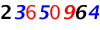
\includegraphics{captcha}
    \caption{Sample captcha}
    \label{fig:sampleCaptcha}
\end{figure}

% todo add these well-known libraries for DS and ML 
% todo extend number of images
 

The goal of this article is to implement several types of classifiers and to assess their accuracy in classifying new elements. Dataset is composed of x images web-scrapped from Spanish postal operator Correos. Details of the scrapping are available at appendix \ref{appendix:tools}. This work will be done mainly in python 3.6, although there will be several steps (i.e Color Removal at chapter \ref{sec:colorRemoval}) that will be performed in bash scripting.\medskip
% todo add github link for this work and for code

This article is structured in the following way: chapter \ref{chap:preprocessing} will explore the steps taken to pre-process the information before actually performing any operations. Next, chapter \ref{chap:processing} will take the pre-processed data to perform classification and then in the chapter \ref{chap:tests} some texts will be conducted, to assess the performance of the generated classifiers. Finally, appendices \ref{appendix:code} and \ref{appendix:tools} will include the generated code and the external tools employed in this work.\medskip

Figure \ref{fig:processPipeline} explains the whole pipeline of this process

\begin{figure}[!htbp]
	\centering
	\begin{tikzpicture}[scale=0.2]
	\tikzstyle{block} = [rectangle, draw, text width=6em, text centered, minimum height=4em]
	\tikzstyle{borderlessblock} = [rectangle, text width=5.5em, text centered, minimum height=4em]
	\tikzstyle{decision} = [diamond, draw,text centered,text width=3em]
	\node [block] (init) {\footnotesize Data origin};
	\node [block,right=1.5em of init] (cross) {\footnotesize Cruce de $P$ padres};
	\node [block,right=1.5em of cross] (eval) {\footnotesize Evaluación de la descendencia};
	\node [block,below=1.5em of eval] (selec) {\footnotesize Selección de los $P$ mejores individuos (entre padres e hijos)};
	\node [block,below=1.5em of selec] (comprob) {\footnotesize Si no hay nuevos individuos tras el cruce, disminuir $L$};
	\node [decision,left=2.45em of comprob] (comprobThres) {\footnotesize $L\leq 0$};
	\node [block,left=1.5em of comprobThres] (restart) {\footnotesize Reiniciar la población y el umbral};
	\draw [->] (init)--(cross);
	\draw [->] (cross)--(eval);
	\draw [->] (eval)--(selec);
	\draw [->] (selec)--(comprob);
	\draw [->] (comprob)--(comprobThres);
	\draw [->] (comprobThres.south)-- node [below,shift={(-3.5em,-0.25em)}] {sí} +(0,-3em) -|(restart.south);
	\draw [->] (comprobThres)-- node [shift={(1em,-2em)}] {no} coordinate(comprobThres-cross) (cross);
	\draw [->] (restart.west)-- +(-5em,0) |- (comprobThres-cross);
	\end{tikzpicture}
	\caption{Process pipeline}
	\label{fig:processPipeline}
\end{figure}
